\documentclass[11pt]{article}

\usepackage[a4paper,margin=1in]{geometry}
\usepackage{amsmath}
\usepackage{booktabs}
\usepackage{float}
\usepackage{graphicx}
\usepackage{hyperref}
\usepackage{listings}
\usepackage{xcolor}
\usepackage{enumitem}
\usepackage{caption}
\emergencystretch=3em
\sloppy

\definecolor{codebg}{RGB}{245,245,245}
\lstset{
  backgroundcolor=\color{codebg},
  basicstyle=\ttfamily\scriptsize,
  breaklines=true,
  frame=single,
  language=Python,
  columns=fullflexible,
  keepspaces=true,
  showstringspaces=false,
  numbers=left,
  numberstyle=\tiny,
  xleftmargin=1.5em
}

\title{Exp-04: When Cache Optimizations Make the Processor Slower}
\author{Deetya Ashish Mehta \\ Roll No: CS23I1032}
\date{\today}

\begin{document}
\maketitle

\begin{abstract}
This report studies four cache optimizations on a five-stage synthetic
data-processing pipeline (ingestion, feature extraction, feature
aggregation, lookup/scoring, result generation): a victim cache, three
prefetch mechanisms (next-line, stride, stream), and a non-blocking cache
with MSHRs. The cache hierarchy is a simplified model of an Intel Xeon
Platinum 8480+ (Sapphire Rapids) core: 48\,KB/12-way L1D, 2\,MB/16-way L2,
15\,MiB/15-way aggregate LLC, 64\,B lines. Every table below is generated
directly from a run of the accompanying simulator and \texttt{\textbackslash
input}ed verbatim, so the numbers in the text match the code exactly. Four
results carry the report's main point, that the right optimization depends
on the workload and that fewer misses does not mean a faster processor.
A distance-1 stride prefetcher cuts the L1 miss rate from 57.4\% to 23.2\%
but makes execution \emph{slower}, because its prefetches arrive with 0\%
timeliness and the extra traffic evicts data still in use. A victim cache
that does almost nothing on the full pipeline (0.008\% faster) removes
61.6\% of the cycles in a purpose-built conflict micro-benchmark, with a
sharp cutoff at exactly (N $-$ ways) entries. Under high interleave
pressure, a stream prefetcher drops the overall L1 miss rate from 99.6\% to
1.0\% while leaving the specific structure that is thrashing completely
unaffected. And in a dedicated MSHR timing model, extra outstanding-miss
slots buy nothing for a dependent pointer-chase but cut an 8-stream
independent workload's time 8$\times$, plateauing exactly at MSHR\,=\,8.
\end{abstract}

\tableofcontents

% =====================================================================
\section{Introduction}
% =====================================================================

Modern processors already ship with a carefully tuned cache hierarchy. The
question this assignment asks is not whether more cache machinery reduces
misses, since it almost always can, but whether it reduces \emph{execution
time}, and under what conditions it stops helping or starts hurting. To
study that question honestly requires a workload realistic enough to
exercise several access patterns at once (streaming, strided, pointer-chasing,
mixed random/regular), and a simulator detailed enough to separate "fewer
misses" from "faster execution" as genuinely different outcomes.

Section~2 describes the simplified processor model. Section~3 describes the
five-stage workload built for this study. Sections~4--9 present the seven
experiment groups: baseline characterization, victim cache, prefetch
mechanisms, prefetch distance, cache pollution and thrashing, and blocking
vs.\ non-blocking caches with MSHRs. Section~10 combines the findings into a
final recommended configuration, and Section~11 checklists every concept the
assignment asks to see demonstrated against the section that demonstrates it.

% =====================================================================
\section{Processor Model and System Parameters}
% =====================================================================

Table~\ref{tab:sysparams} lists the simplified 8-core-subset model used
throughout. Capacities and line size follow the assignment exactly (L1
48\,KB, L2 2\,MB, LLC 1.875\,MB/core $\times$ 8 = 15\,MiB aggregate, 64\,B
lines); associativity, per-level latency, and DRAM latency are reasoned
choices for parameters the assignment leaves open, and are meant as an
architectural reference rather than a bit-for-bit reproduction of the real
chip, which the assignment states is acceptable.

\begin{table}[H]\centering
\begin{tabular}{lll}\toprule
Level & Parameters & Rationale \\ \midrule
L1D & 48\,KB, 12-way, 64 sets, 5 cyc & Golden Cove L1D is 48\,KB/12-way \\
L2  & 2\,MB, 16-way, 2048 sets, 16 cyc & assignment-given capacity \\
LLC & 15\,MiB (aggregate), 15-way, 16384 sets, 60 cyc & 8$\times$1.875\,MB/core \\
DRAM & 200 cyc & illustrative SPR/DDR5-class latency \\
Victim cache & fully associative, +3 cyc over L1 hit & small, parallel lookup \\
Line size & 64\,B (all levels) & assignment-given \\ \bottomrule
\end{tabular}
\caption{Simplified processor/cache model used for every experiment.}
\label{tab:sysparams}
\end{table}

All three set counts (64, 2048, 16384) come out to exact powers of two given
these capacities, associativities, and line size. The 15-way LLC looks
unusual on paper, but it is exactly what $15\,\text{MiB}/64\,\text{B} =
245760$ lines factors into with $16384 = 2^{14}$ sets, and real Intel LLC
slices are often non-power-of-two-way for the same reason.

\textbf{Timing model.} Every experiment except Section~\ref{sec:mshr} uses a
cumulative, serial latency model: an access that misses in L1 and hits in L2
costs $L1_{lat}+L2_{lat}$; a full miss costs $L1_{lat}+L2_{lat}+LLC_{lat}+DRAM_{lat}$.
This is a single-outstanding-request (blocking) model, adequate for every
question about miss rates, pollution, and prefetch effectiveness, but blind
to memory-level parallelism by construction: run through it, a dependent
pointer-chase and eight independent streams of the same size come out to the
identical total clock, since the model has no notion of two misses ever
being outstanding at once. That is exactly why Section~\ref{sec:mshr} uses a
separate, request-level timing model instead.

Prefetched lines are inserted into the cache at issue time, so an early or
wasted prefetch correctly participates in LRU/eviction bookkeeping the
moment it is fetched. Each prefetched line also carries a predicted arrival
clock; a demand access that arrives before that clock still pays the
remaining wait, which is what makes a "late" prefetch measurable. Every
prefetcher here targets L1 directly (prefetch requests walk the full
hierarchy and fill up to L1), so L1 pollution is visible rather than hidden
behind L2/LLC.

% =====================================================================
\section{Workload}
% =====================================================================

A five-stage pipeline is implemented in \texttt{src/workload.py} as an
address-stream generator, in the same style as the Exp-01/Exp-03
simulators: no data values are modeled, only the addresses a real
implementation would touch. That is enough, since every phenomenon under
study here is about where and when memory is accessed, not what arithmetic
runs on it.

\begin{enumerate}[leftmargin=1.6em]
\item \textbf{Data Ingestion.} A sequential scan of an 80{,}000-record array
(128\,B/record, 2 cache lines each), $\approx$9.8\,MB and touched once per
record, so there is no temporal reuse in the record stream itself. A small
4\,KB metadata block is re-touched twice per record, standing in for reused
processing parameters.
\item \textbf{Feature Extraction.} Re-reads the same record array at a
configurable record-level stride, from contiguous up to arbitrarily large,
touching a fixed 60{,}000 records regardless of stride so useful work stays
constant while only the address pattern changes. Forward and backward
traversal are both supported.
\item \textbf{Feature Aggregation.} A small 512-entry (4\,KB) accumulator,
updated once every 4 input records. This is the workload's "small,
frequently reused state" structure, central to Section~\ref{sec:pollution}.
\item \textbf{Lookup and Scoring.} A 200{,}000-entry ($\approx$6.1\,MB) index
accessed with a 60/40 mix of pseudo-random indices and a periodic,
partially-predictable regular component.
\item \textbf{Result Generation.} Two variants of equal footprint
($\approx$2.56\,MB, 40{,}000 nodes): a dependent pointer-chase (visitation
order is a precomputed random cyclic permutation, the standard way to model
pointer-chasing without simulating memory contents) and $K=8$ independent
chains, round-robin interleaved. Independence here means stream $k$ never
waits on stream $j$'s outstanding request, but each stream is still
internally a dependent chain, which is what gives memory-level parallelism a
finite bound ($K$) instead of an unrealistic unbounded one.
\end{enumerate}

The full pipeline runs stages 1--5 back to back through one simulator
instance, without clearing cache state between stages. Section~\ref{sec:baseline}
shows this directly: Extraction's LLC miss rate is 0.00\% because it re-reads
data Ingestion just streamed through the LLC.

% =====================================================================
\section{Experiment A: Baseline Characterization}
\label{sec:baseline}
% =====================================================================

Table~\ref{tab:expA} and Figure~\ref{fig:expA} give the per-stage miss rate
and AMAT of the unmodified pipeline: no victim cache, no prefetching.

\begin{figure}[H]\centering
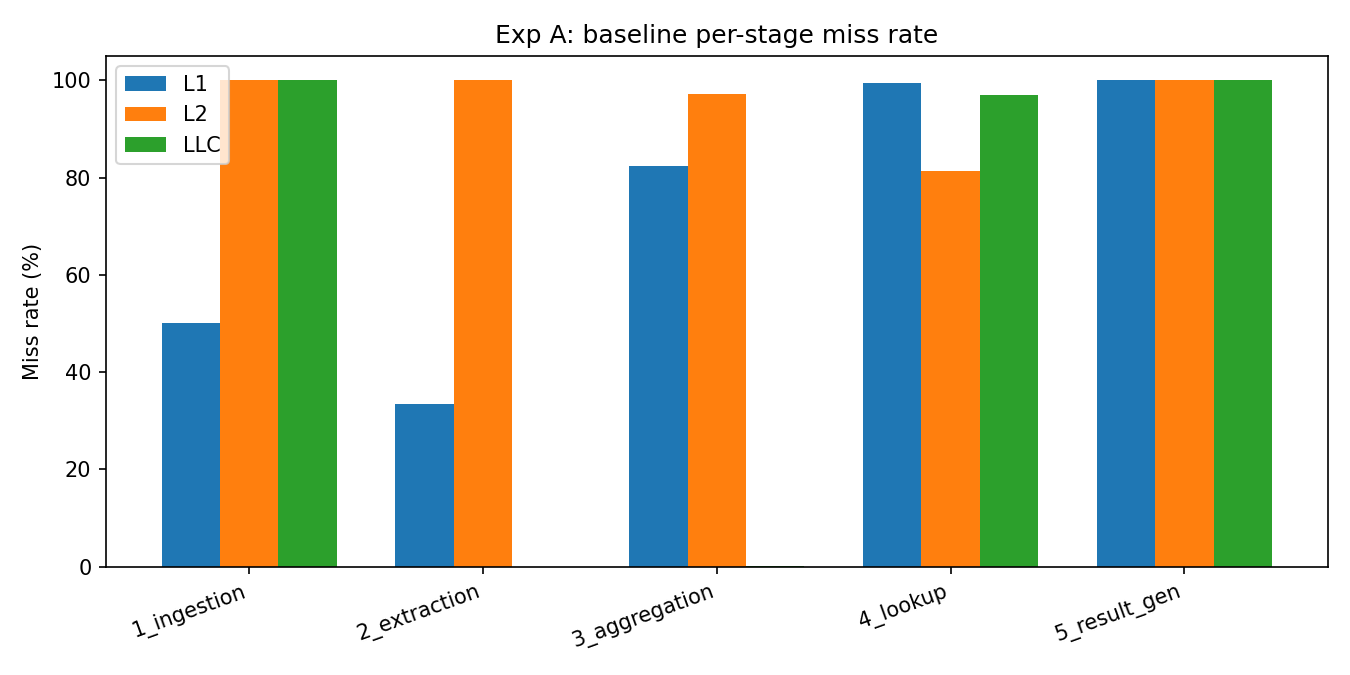
\includegraphics[width=0.85\textwidth]{../results/plots/expA_stage_miss_rates.png}
\caption{Baseline per-stage miss rate by cache level.}
\label{fig:expA}
\end{figure}

\begin{table}[H]\centering\small
\begin{tabular}{lrrrrrr}\toprule
Stage & Accesses & L1 Miss\% & L2 Miss\% & LLC Miss\% & DRAM Acc. & AMAT \\ \midrule
1\_ingestion & 320,000 & 50.00 & 100.00 & 100.00 & 160,002 & 143.00 \\
2\_extraction & 180,000 & 33.33 & 100.00 & 0.00 & 0 & 30.33 \\
3\_aggregation & 100,000 & 82.41 & 97.15 & 0.08 & 64 & 66.35 \\
4\_lookup & 60,000 & 99.40 & 81.35 & 96.91 & 47,020 & 226.16 \\
5\_result\_gen & 40,000 & 100.00 & 100.00 & 100.00 & 40,000 & 281.00 \\
\bottomrule\end{tabular}
\caption{Exp A: baseline per-stage characterization (no victim cache, no prefetching).}
\label{tab:expA}\end{table}

\begin{table}[H]\centering\small
\begin{tabular}{lrrr}\toprule
Stage segment & Accesses & L1 Miss\% & AMAT \\ \midrule
1\_ingestion\_cold\_0-20pct & 64,000 & 50.00 & 143.01 \\
1\_ingestion\_steady\_20-100pct & 256,000 & 50.00 & 143.00 \\
2\_extraction\_cold\_0-20pct & 36,000 & 33.33 & 30.33 \\
2\_extraction\_steady\_20-100pct & 144,000 & 33.33 & 30.33 \\
3\_aggregation\_cold\_0-20pct & 20,000 & 82.59 & 67.05 \\
3\_aggregation\_steady\_20-100pct & 80,000 & 82.37 & 66.18 \\
4\_lookup\_cold\_0-20pct & 12,000 & 99.42 & 269.19 \\
4\_lookup\_steady\_20-100pct & 48,000 & 99.40 & 215.40 \\
5\_result\_gen\_cold\_0-20pct & 8,000 & 100.00 & 281.00 \\
5\_result\_gen\_steady\_20-100pct & 32,000 & 100.00 & 281.00 \\
\bottomrule\end{tabular}
\caption{Exp A: first 20\% (cold) vs. remaining 80\% (steady-state) of each stage.}
\label{tab:expA-cold}\end{table}



Ingestion is 100\% miss at L2 and LLC, and 50\% miss at L1, matching the two
per-record lines missing and the two metadata touches after the first
hitting: a clean capacity-miss stream. Extraction's LLC miss rate is 0.00\%,
since it re-reads the same 9.8\,MB array Ingestion just finished streaming
through and the 15\,MiB LLC can still hold essentially all of it, which is
direct evidence of state carried across stages. Aggregation's L1 miss rate
(82.4\%) is higher than Extraction's despite reusing the same record array,
because it interleaves that scan with writes to \texttt{agg\_state}, which
foreshadows Section~\ref{sec:pollution}. Lookup is the worst stage by AMAT
(226 cycles): a $\approx$6.1\,MB structure touched for the first time, 60\%
randomly, so even the LLC only catches 3.1\% of the L2-missing traffic.
Result Generation is a clean 100\% miss at every level by design.

Table~\ref{tab:expA-cold} splits each stage into its first 20\% ("cold")
and remaining 80\% ("steady-state"). Ingestion and Extraction show a small
early-stage AMAT bump while the metadata block and front of the record array
are still filling in; Lookup and Result Generation show almost no
cold/steady difference, since neither working set is ever revisited within
one pass.

% =====================================================================
\section{Experiment B: Victim Cache}
\label{sec:victim}
% =====================================================================

Table~\ref{tab:expB} sweeps victim-cache size against the full pipeline.

\begin{figure}[H]\centering
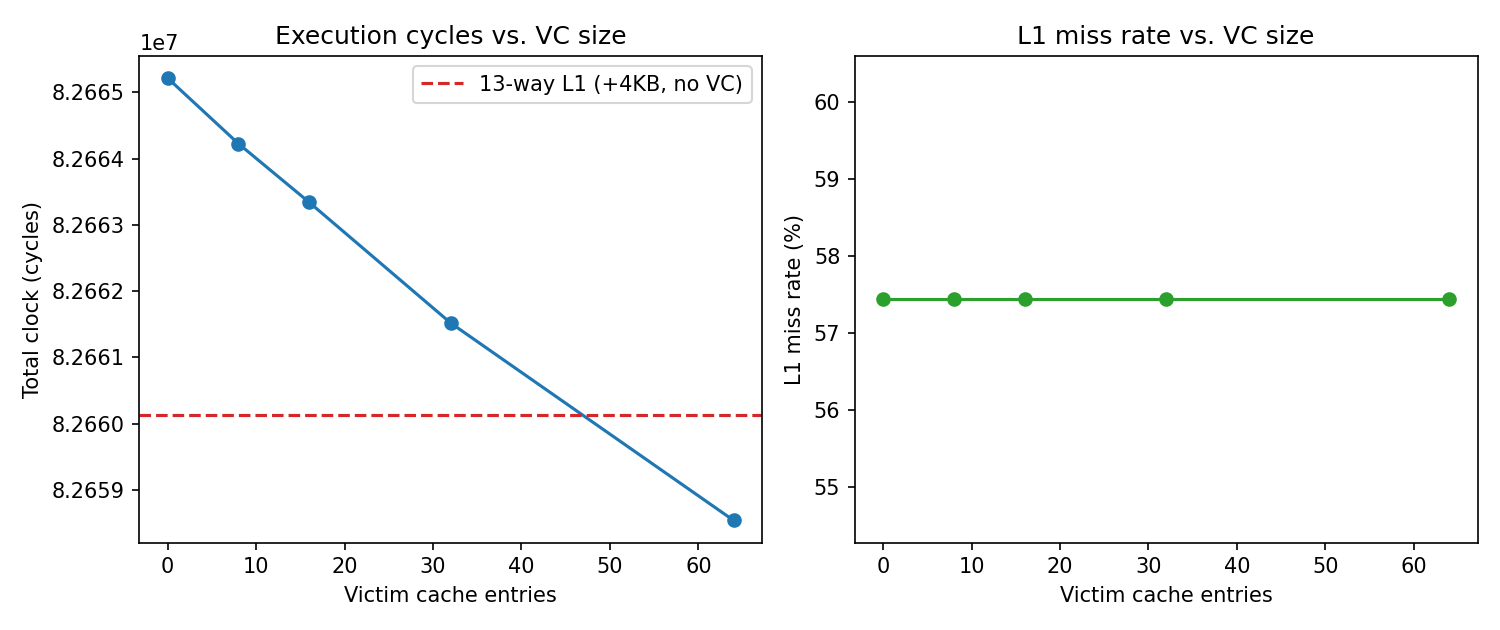
\includegraphics[width=\textwidth]{../results/plots/expB_victim_cache.png}
\caption{Full-pipeline victim-cache sweep: execution cycles and L1 miss
rate vs.\ victim-cache size, with the equal-extra-storage 13-way L1
alternative shown as a reference line.}
\label{fig:expB}
\end{figure}

\begin{table}[H]\centering\small
\begin{tabular}{rrrrrr}\toprule
VC entries & Extra bytes & Clock (cyc) & L1 Miss\% & VC hits & AMAT \\ \midrule
0 & 0 & 82,665,212 & 57.44 & 0 & 118.09 \\
8 & 512 & 82,664,224 & 57.44 & 76 & 118.09 \\
16 & 1,024 & 82,663,340 & 57.44 & 144 & 118.09 \\
32 & 2,048 & 82,661,520 & 57.44 & 284 & 118.09 \\
64 & 4,096 & 82,658,543 & 57.44 & 513 & 118.08 \\
\midrule 13-way L1 (+4KB, no VC) & 4{,}096 & 82,660,140 & 57.39 & -- & 118.09 \\
\bottomrule\end{tabular}
\caption{Exp B: victim-cache size sweep vs. an equal-extra-storage associativity increase.}
\label{tab:expB}\end{table}



On the full pipeline a victim cache is essentially invisible: even 64
entries only shave 0.008\% off total cycles, and move the L1 miss rate by
less than 0.01 points. This is a real result, not a bug. The full pipeline's
misses are overwhelmingly cold or capacity misses on datasets far larger
than any cache (Section~\ref{sec:baseline}), and a victim cache targets
\emph{conflict} misses specifically, a handful of addresses repeatedly
aliasing to the same set despite the working set nominally fitting. A
one-pass streaming scan almost never produces that signature. The
equal-extra-storage alternative, an L1 widened to 13-way (the same +4\,KB
as the 64-entry victim cache), does marginally better than the victim cache
here (82{,}660{,}140 vs.\ 82{,}658{,}543 cycles): with almost no
conflict-miss opportunity to recover, spending the extra 4\,KB as
unconditional L1 capacity is at least as good as reserving it for
victim-only overflow.

To show the behavior a victim cache is actually built for, a supplementary
micro-benchmark isolates it directly: 15 addresses, all mapping to the same
12-way L1 set, accessed round-robin for 3000 rounds, a classic pathological
pattern in which every access misses once the address count exceeds the
set's associativity.

\begin{figure}[H]\centering
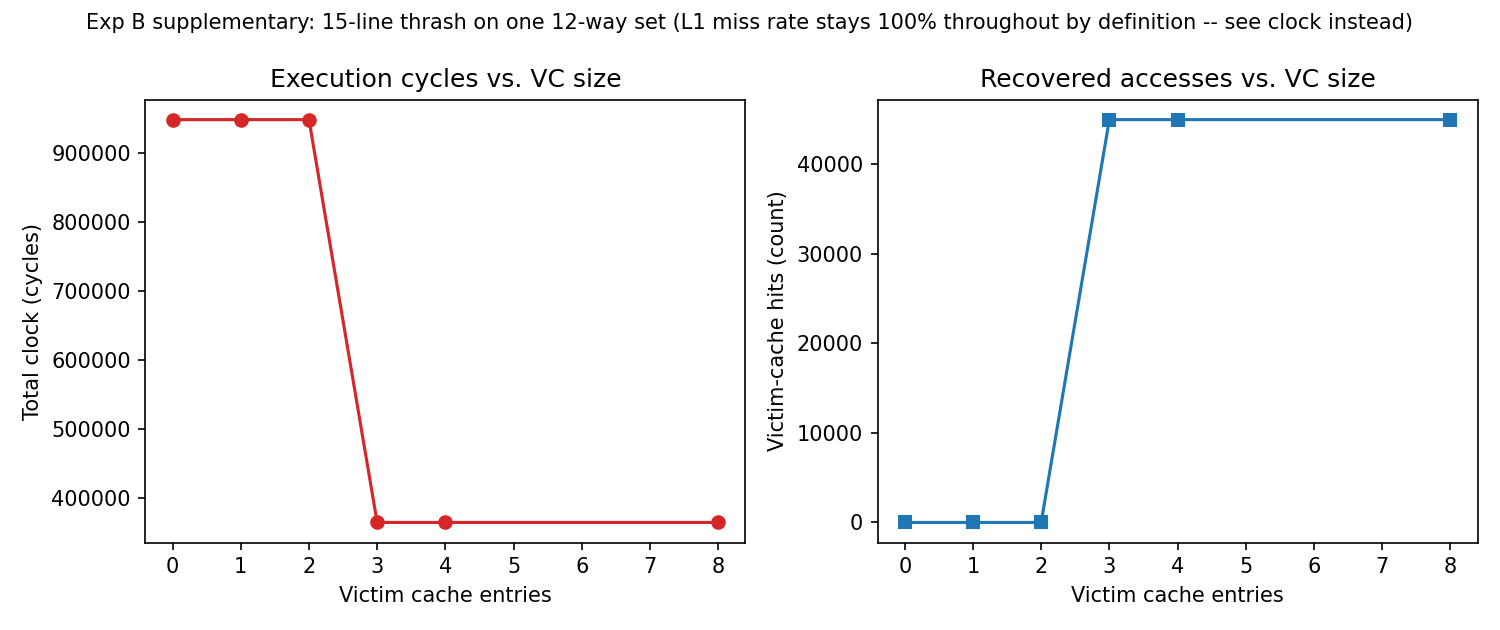
\includegraphics[width=0.95\textwidth]{../results/plots/expB_conflict_microbench.png}
\caption{Conflict micro-benchmark: execution cycles and recovered
(victim-cache-hit) accesses vs.\ victim-cache size. L1 miss rate stays flat
at 100\% throughout by definition, since a victim-cache hit is still an L1
miss, even as cycles fall sharply.}
\label{fig:expB-conflict}
\end{figure}

\begin{table}[H]\centering\small
\begin{tabular}{rrrr}\toprule
VC entries & L1 Miss\% & Clock (cyc) & VC hits \\ \midrule
0 & 100.00 & 948,900 & 0 \\
1 & 100.00 & 948,900 & 0 \\
2 & 100.00 & 948,900 & 0 \\
3 & 100.00 & 364,095 & 44,985 \\
4 & 100.00 & 364,095 & 44,985 \\
8 & 100.00 & 364,095 & 44,985 \\
\bottomrule\end{tabular}
\caption{Exp B supplementary: 15 addresses round-robin thrashing one 12-way L1 set.}
\label{tab:expB-conflict}\end{table}



Here the threshold is sharp: 0, 1, and 2 victim entries give zero
improvement (clock stays at 948{,}900 cycles), but at exactly VC\,=\,3,
which is $N - \text{ways} = 15 - 12$, clock drops to 364{,}095 cycles (a
61.6\% reduction) and 44{,}985 accesses become victim-cache hits. VC\,=\,4
and VC\,=\,8 give no further improvement at all: once the victim cache is
exactly large enough to hold the overflow the primary cache cannot, more
capacity is wasted. This is the answer the full-pipeline sweep could not
give: a victim cache recovers data when a small number of addresses thrash
one set, and its useful capacity stops exactly at (contending addresses $-$
associativity).

Worth noting: the micro-benchmark's L1 miss rate reads 100\% in every row of
the underlying data, even where clock drops 61.6\%, because a victim-cache
hit is still an L1 miss by definition. A raw miss-rate number at one level
can look unchanged while execution time moves by more than half.

% =====================================================================
\section{Experiment C: Prefetch Mechanisms and Effectiveness}
\label{sec:prefetch}
% =====================================================================

Three prefetchers, implemented in \texttt{src/cache\_core.py}, are applied
to the complete workload rather than hand-picked to the stage each suits
best: \textbf{next-line} (stateless, on every L1 miss to line $L$ prefetch
$L+1$), \textbf{stride} (per-stream two-delta detector, one prefetch issued
\texttt{distance} strides ahead once confirmed), and \textbf{stream}
(per-stream run-ahead engine, requiring two consecutive matching deltas to
confirm, then maintaining a \texttt{distance}-line run-ahead window).
"Per-stream" state is keyed on the workload's logical stream tags
(\texttt{ingest\_records}, \texttt{extract}, \texttt{lookup}, \ldots), the
simulator-level stand-in for the per-PC stride tables real hardware uses.

\begin{figure}[H]\centering
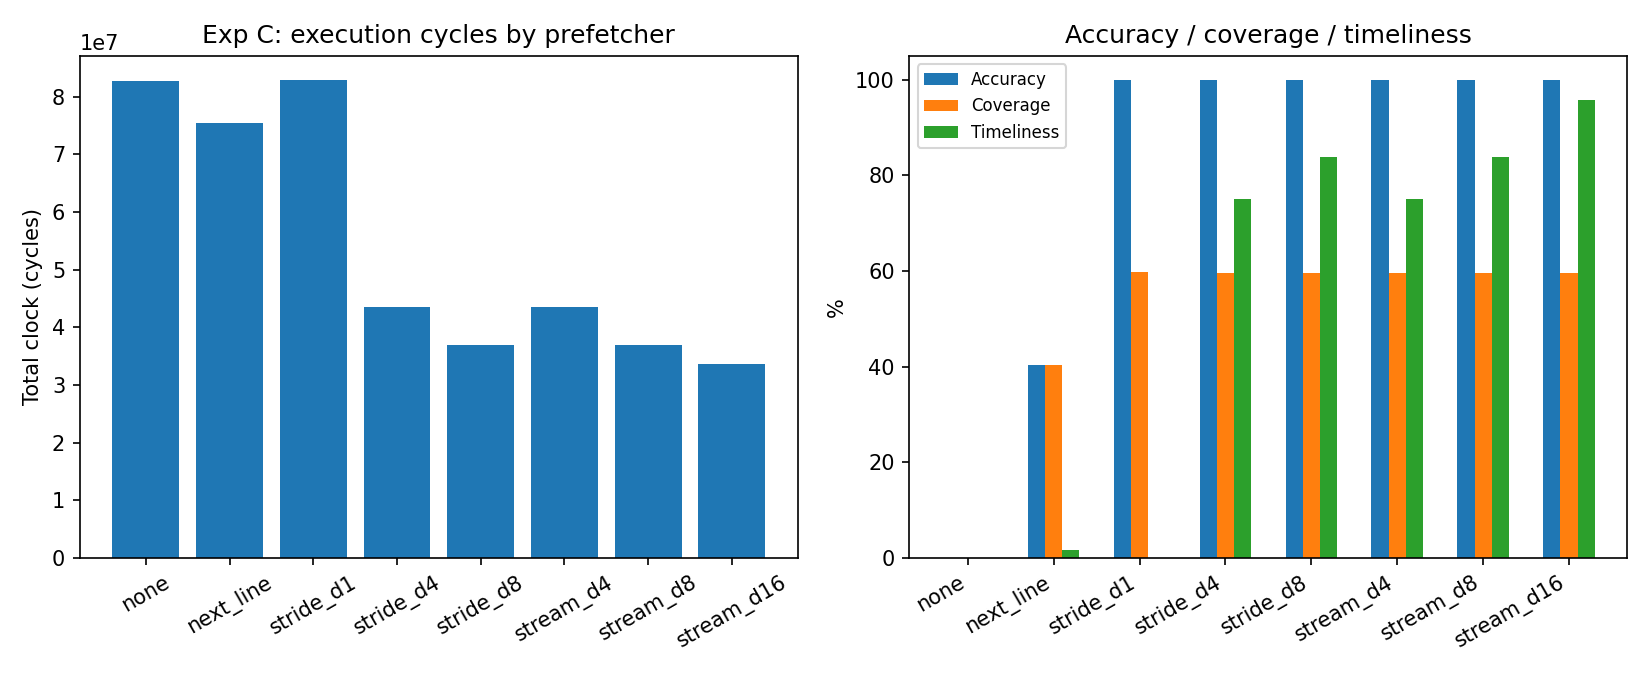
\includegraphics[width=\textwidth]{../results/plots/expC_prefetchers.png}
\caption{Left: total execution cycles by prefetcher. Right: accuracy,
coverage, and timeliness (\%) by prefetcher.}
\label{fig:expC}
\end{figure}

\begin{table}[H]\centering\small
\begin{tabular}{lrrrrrr}\toprule
Prefetcher & Clock (cyc) & L1 Miss\% & Accuracy\% & Coverage\% & Timeliness\% & Issued \\ \midrule
none & 82,665,212 & 57.44 & 0.0 & 0.0 & 0.0 & 0 \\
next\_line & 75,510,773 & 34.57 & 40.4 & 40.4 & 1.6 & 402,223 \\
stride\_d1 & 82,920,183 & 23.15 & 100.0 & 59.7 & 0.0 & 240,060 \\
stride\_d4 & 43,439,008 & 23.16 & 100.0 & 59.7 & 75.0 & 240,105 \\
stride\_d8 & 36,863,516 & 23.16 & 100.0 & 59.7 & 83.9 & 240,107 \\
stream\_d4 & 43,444,992 & 23.16 & 100.0 & 59.7 & 75.0 & 239,998 \\
stream\_d8 & 36,867,718 & 23.16 & 100.0 & 59.7 & 83.9 & 240,006 \\
stream\_d16 & 33,689,342 & 23.17 & 100.0 & 59.7 & 95.8 & 240,022 \\
\bottomrule\end{tabular}
\caption{Exp C: prefetch mechanism comparison, full pipeline.}
\label{tab:expC}\end{table}



Accuracy, coverage, and timeliness are computed as specified: accuracy is
useful prefetches over issued prefetches; coverage is useful prefetches over
baseline (no-prefetch) demand misses; timeliness is the fraction of useful
prefetches that had already arrived by the time they were referenced.
Prefetch traffic (DRAM/cache accesses generated by prefetch requests) is
counted completely separately from demand traffic.

The central finding is in the \texttt{stride\_d1} row: 100.0\% accuracy, L1
miss rate more than halved (57.4\% $\to$ 23.2\%), yet total cycles rise
slightly, from 82{,}665{,}212 to 82{,}920{,}183. Every issued prefetch
eventually gets used, but timeliness is 0.0\%: at distance 1 the prefetch
target is only one stride ahead of the access that triggered it, so the
demand stream catches up to (and still waits out) essentially every
in-flight prefetch, while the extra traffic still evicts data that was
genuinely still in use. High accuracy and a large drop in the raw miss count
provide no performance benefit here, because a prefetch only pays off by
hiding latency behind other work, and distance 1 leaves nothing to hide it
behind.

\texttt{next\_line} shows the opposite failure mode: accuracy only 40.4\%
and timeliness 1.6\%, since it fires unconditionally regardless of whether
the current stream is even sequential. It does reasonably well on
Ingestion's two-line-per-record scan (field 0 and field 8 sit on adjacent
lines), but is essentially blind guessing on Lookup's mostly-random index
stream. It still nets a win overall (82.67M $\to$ 75.51M cycles), purely
because Ingestion's regularity outweighs its failures elsewhere, but it is
clearly the least reliable of the three mechanisms.

% =====================================================================
\section{Experiment D: Prefetch Distance and Unintended Effects}
\label{sec:distance}
% =====================================================================

Table~\ref{tab:expD} and Figure~\ref{fig:expD} sweep prefetch distance for
stride and stream across the full pipeline, including the no-prefetch
reference point (distance 0).

\begin{figure}[H]\centering
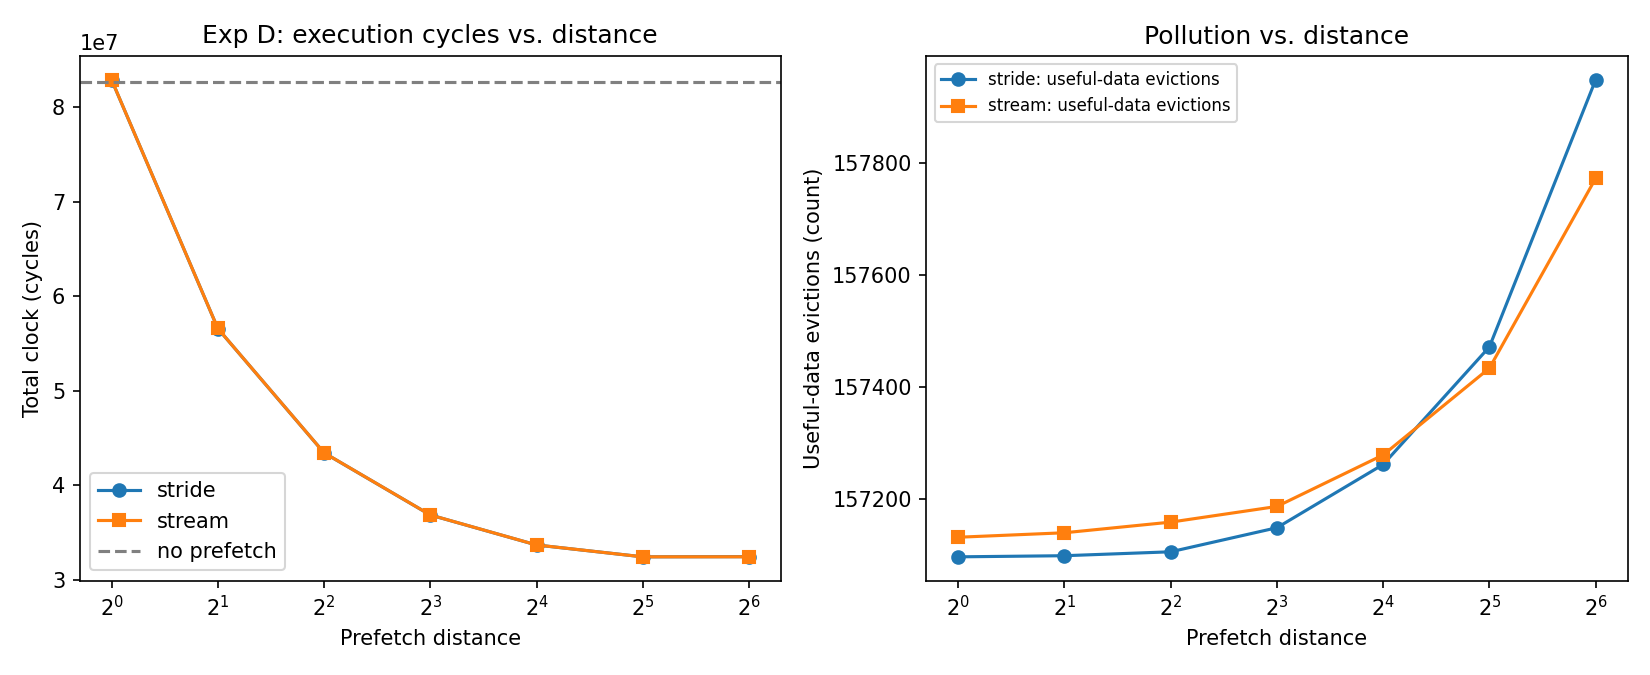
\includegraphics[width=\textwidth]{../results/plots/expD_distance_sweep.png}
\caption{Left: execution cycles vs.\ prefetch distance (log scale). Right:
useful-data evictions (pollution) vs.\ distance.}
\label{fig:expD}
\end{figure}

\begin{table}[H]\centering\small
\begin{tabular}{lrrrrr}\toprule
Kind & Distance & Clock (cyc) & L1 Miss\% & Wasted-evicted PF & Useful-data evictions \\ \midrule
none & 0 & 82,665,212 & 57.44 & 0 & 765,916 \\
stride & 1 & 82,920,183 & 23.15 & 248,860 & 157,097 \\
stride & 2 & 56,600,572 & 23.15 & 248,909 & 157,099 \\
stride & 4 & 43,439,008 & 23.16 & 248,973 & 157,106 \\
stride & 8 & 36,863,516 & 23.16 & 248,985 & 157,149 \\
stride & 16 & 33,685,428 & 23.18 & 249,027 & 157,262 \\
stride & 32 & 32,432,768 & 23.20 & 249,061 & 157,472 \\
stride & 64 & 32,449,932 & 23.26 & 249,080 & 157,949 \\
stream & 1 & 82,922,825 & 23.15 & 248,761 & 157,132 \\
stream & 2 & 56,603,970 & 23.15 & 248,763 & 157,140 \\
stream & 4 & 43,444,992 & 23.16 & 248,771 & 157,159 \\
stream & 8 & 36,867,718 & 23.16 & 248,791 & 157,187 \\
stream & 16 & 33,689,342 & 23.17 & 248,826 & 157,279 \\
stream & 32 & 32,431,948 & 23.20 & 248,894 & 157,434 \\
stream & 64 & 32,437,372 & 23.25 & 248,969 & 157,773 \\
\bottomrule\end{tabular}
\caption{Exp D: prefetch distance sweep, full pipeline (distance 0 = no prefetch).}
\label{tab:expD}\end{table}



For both mechanisms, distance 1 is a net loss against no prefetching;
distance 2 already recovers to a large net win (56.6M cycles); cycles keep
falling through distance 32 (32.43M cycles, timeliness 95--96\%) as
prefetches increasingly arrive with time to hide the miss latency; and
distance 64 is very slightly worse than distance 32 for both mechanisms
(32.45M vs.\ 32.43M stride, 32.44M vs.\ 32.43M stream), even though its raw
miss count is marginally lower still. At that point the run-ahead window is
far enough ahead of the demand stream that some of what it fetches is
evicted before use, adding traffic without adding benefit. Together these
three distances trace the "too late / just right / too aggressive" arc
inside one mechanism.

A demand miss costs the full serial latency ($\approx$281 cycles here)
whether or not a prefetch was issued for that line. A prefetch only turns
that cost into a win if it completes before the demand needs it and does
not itself displace data that would otherwise still be there. Reducing the
demand-miss count is necessary but not sufficient for reducing execution
time: accuracy alone only says a prefetch was eventually useful, not that it
was useful in time, and coverage says nothing about what it evicted along
the way.

% =====================================================================
\section{Experiment E: Cache Pollution and Thrashing}
\label{sec:pollution}
% =====================================================================

Sections~\ref{sec:baseline}--\ref{sec:distance} show pollution as a side
effect; this experiment builds it on purpose. Ingestion, Extraction, and
Aggregation run genuinely interleaved at record granularity rather than
stage by stage: for every record, two ingestion lines are touched, then
\texttt{pressure} fresh, never-before-touched filler lines are touched
(standing in for continuously arriving input), and every 4th record also
touches the small, hot \texttt{agg\_state} array. \texttt{pressure} directly
and monotonically controls how much foreign traffic separates one touch of
the hot state from the next. An earlier version of this experiment drove
pressure through a modular record stride instead of a never-repeating
filler region, and produced a non-monotonic curve caused by the stride
sharing a factor with the array length -- a reminder of how easily a
synthetic "pressure" generator can build in unintended extra reuse.

\begin{figure}[H]\centering
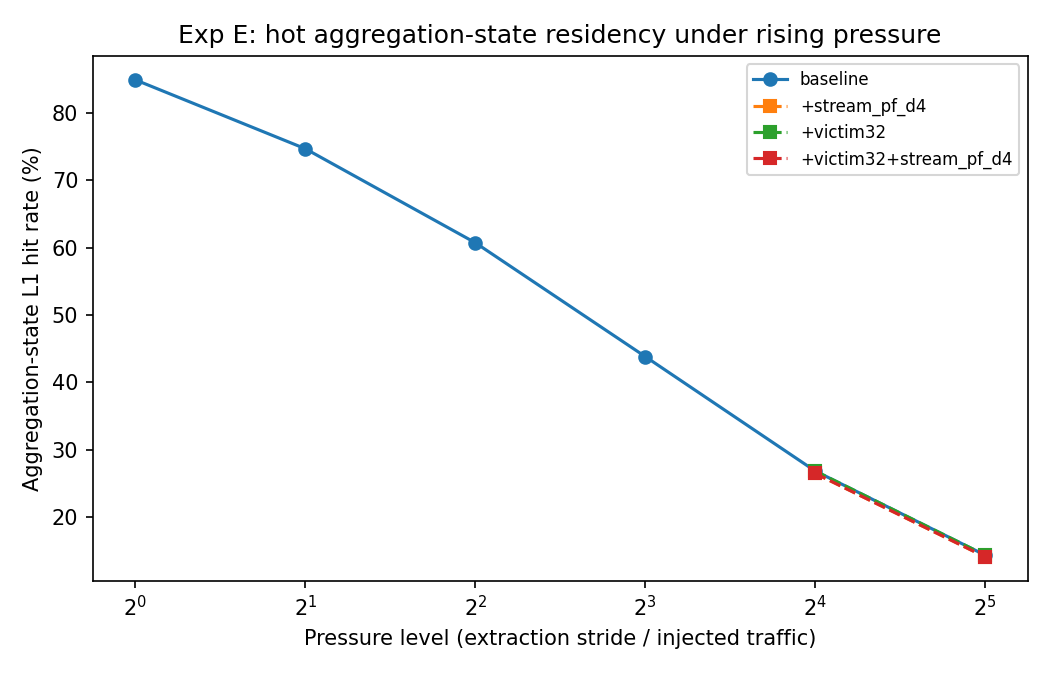
\includegraphics[width=0.75\textwidth]{../results/plots/expE_pollution_thrashing.png}
\caption{Aggregation-state L1 hit rate vs.\ pressure, baseline and with
victim-cache / stream-prefetcher mitigation at the two highest pressure
levels.}
\label{fig:expE}
\end{figure}

\begin{table}[H]\centering\small
\begin{tabular}{rrr}\toprule
Pressure level & Aggregation-state L1 hit\% & Overall L1 Miss\% \\ \midrule
1 & 84.92 & 93.47 \\
2 & 74.69 & 95.61 \\
4 & 60.73 & 97.57 \\
8 & 43.82 & 98.93 \\
16 & 26.82 & 99.63 \\
32 & 14.32 & 99.90 \\
\bottomrule\end{tabular}
\caption{Exp E: baseline aggregation-state residency under rising interleave pressure.}
\label{tab:expE-baseline}\end{table}

\begin{table}[H]\centering\small
\begin{tabular}{rlrr}\toprule
Pressure & Mitigation & Aggregation-state L1 hit\% & Overall L1 Miss\% \\ \midrule
16 & +victim32 & 26.82 & 99.63 \\
16 & +stream\_pf\_d4 & 26.46 & 1.01 \\
16 & +victim32+stream\_pf\_d4 & 26.46 & 1.01 \\
32 & +victim32 & 14.32 & 99.90 \\
32 & +stream\_pf\_d4 & 14.06 & 0.63 \\
32 & +victim32+stream\_pf\_d4 & 14.06 & 0.63 \\
\bottomrule\end{tabular}
\caption{Exp E: does the victim cache and/or prefetching alleviate high-pressure thrashing?}
\label{tab:expE-mitigation}\end{table}



The aggregation state's own L1 hit rate falls, monotonically, from 84.9\% at
the lowest pressure to 14.3\% at the highest, while the workload's overall
L1 miss rate keeps climbing toward $\approx$100\% throughout regardless of
pressure, since it is dominated by the ever-growing, inherently-cold filler
stream. This is the distinction between a large working set and repeatedly
destroyed cache residency: the aggregation state itself is tiny (512
entries, 4\,KB, it would trivially fit in L1 alone) and is never too large
for the cache on its own. What destroys its hit rate is the volume of
unrelated traffic injected between two of its own touches, which at high
pressure exceeds the L1's associativity in nearly every set before the
state is next needed.

Do the other mechanisms help or intensify this? They answer differently. A
32-entry victim cache changes nothing: at pressure 16 and 32 both the
aggregation-state hit rate and overall miss rate are identical to baseline.
A continuous flood of always-cold filler lines touching essentially every
set overwhelms 32 entries; this is capacity pressure spread broadly across
the cache, not the concentrated same-set conflict pattern
Section~\ref{sec:victim}'s micro-benchmark isolates. A distance-4 stream
prefetcher does the opposite: overall L1 miss rate collapses from 99.6\% to
1.0\% at pressure 16 (99.9\% $\to$ 0.63\% at pressure 32), since the filler
stream is purely sequential, exactly what a stream prefetcher is built for.
But the aggregation state's own hit rate is essentially unchanged
(26.82\% $\to$ 26.46\% at pressure 16, if anything marginally worse, since
the prefetcher adds still more traffic competing for the same sets). A
mechanism can be a large net win for a workload as a whole while being
irrelevant, or mildly counter-productive, for one specific structure inside
it.

% =====================================================================
\section{Experiment F: Blocking vs.\ Non-Blocking Cache and MSHRs}
\label{sec:mshr}
% =====================================================================

The blocking clock used everywhere above cannot show memory-level
parallelism by construction: it sums per-access latencies in program order
and has no notion of two misses being outstanding at once, so the
dependent-chain and independent-streams variants of Result Generation come
out to the same total clock through it. \texttt{src/mlp\_model.py}
reclassifies the same access stream (hit/miss and per-access service
latency, taken from one blocking-model pass) through an explicit MSHR-timing
model instead: a request needs a free MSHR slot to start service, and stalls
if all \texttt{mshr\_count} slots are busy; within one logical stream, the
next access cannot issue before the previous access on that same stream
completes. That last rule is what makes "independent streams" independent
of \emph{each other} while still leaving each stream's own requests properly
serialized, so achievable parallelism is bounded by $K = 8$ rather than
unrealistically unbounded.

\begin{figure}[H]\centering
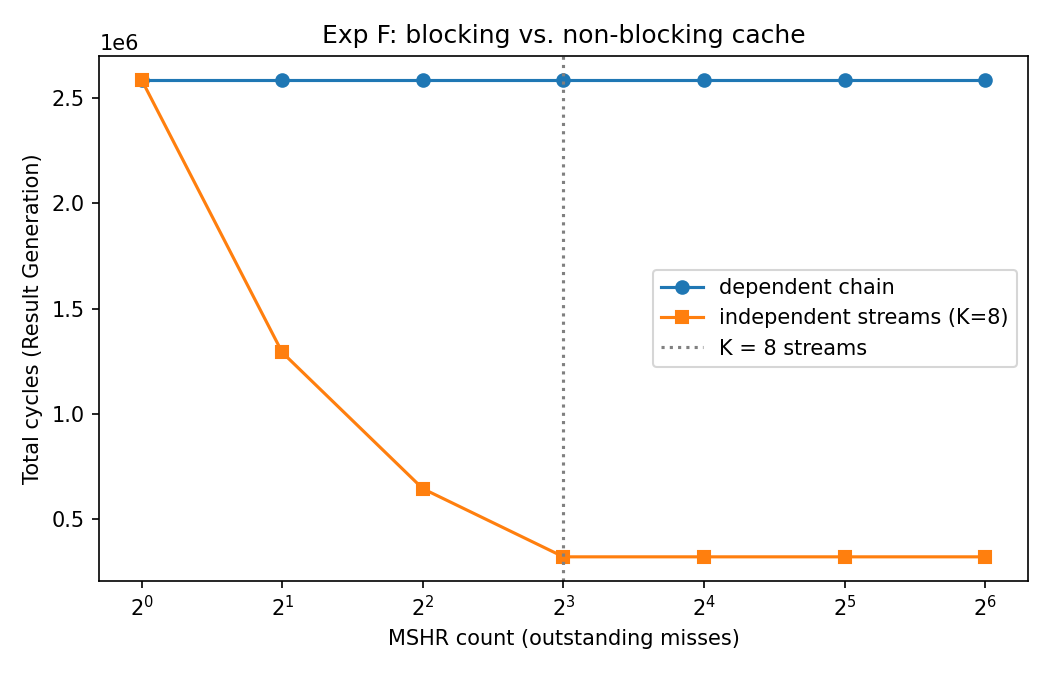
\includegraphics[width=0.75\textwidth]{../results/plots/expF_mshr_sweep.png}
\caption{Total Result-Generation execution cycles vs.\ MSHR count
(log-scale x-axis), dependent chain vs.\ 8 independent streams.}
\label{fig:expF}
\end{figure}

\begin{table}[H]\centering\small
\begin{tabular}{rrr}\toprule
MSHRs & Dependent chain (cyc) & Independent streams (cyc) \\ \midrule
1 & 2,584,000 & 2,584,000 \\
2 & 2,584,000 & 1,292,001 \\
4 & 2,584,000 & 646,003 \\
8 & 2,584,000 & 323,007 \\
16 & 2,584,000 & 323,007 \\
32 & 2,584,000 & 323,007 \\
64 & 2,584,000 & 323,007 \\
\bottomrule\end{tabular}
\caption{Exp F: total Result-Generation execution cycles vs. MSHR count.}
\label{tab:expF}\end{table}



The dependent chain is flat at 2{,}584{,}000 cycles from MSHR\,=\,1 through
MSHR\,=\,64: extra outstanding-miss slots cannot help a request stream that
never has more than one independent request in flight, since the next
address is unknown until the current one returns. The independent-streams
variant instead falls by almost exactly half with every doubling of MSHR
count (2{,}584{,}000 $\to$ 1{,}292{,}001 $\to$ 646{,}003 $\to$ 323{,}007 for
MSHR\,=\,1,2,4,8), textbook memory-latency hiding, and then plateaus exactly
at MSHR\,=\,8, matching $K=8$ streams precisely: MSHR\,=\,16, 32, and 64 all
give the identical 323{,}007 cycles, since at most 8 requests can ever be
simultaneously ready to issue.

MSHRs (miss status holding registers) are what make a non-blocking cache
non-blocking: each tracks one in-flight miss so the pipeline can keep
accepting new requests instead of stalling behind the first one.
Outstanding misses are exactly the requests those MSHRs track; a request
that finds none free must itself stall, and MSHR\,=\,1 is simply the
blocking case, confirmed above since the independent-streams row at
MSHR\,=\,1 matches the dependent chain exactly. Memory-level parallelism is
the amount of concurrent, mutually-independent outstanding-miss activity a
request stream can offer; memory-latency hiding is what non-blocking
hardware does with that opportunity, overlapping one miss's wait behind
another's. Extra MSHRs help the independent-streams workload far more than
the dependent one because only the former has parallelism to exploit, and
they stop helping the moment their count reaches the workload's own ceiling
on simultaneously-ready requests, a property of the algorithm that no amount
of extra buffering can raise.

% =====================================================================
\section{Final Performance Analysis and Recommendation}
% =====================================================================

Table~\ref{tab:expG} compares four full-pipeline configurations: baseline;
victim-cache-only (64 entries, best from Section~\ref{sec:victim});
prefetch-only (stream at distance 16, best single mechanism from
Sections~\ref{sec:prefetch}--\ref{sec:distance}); and both combined.

\begin{figure}[H]\centering
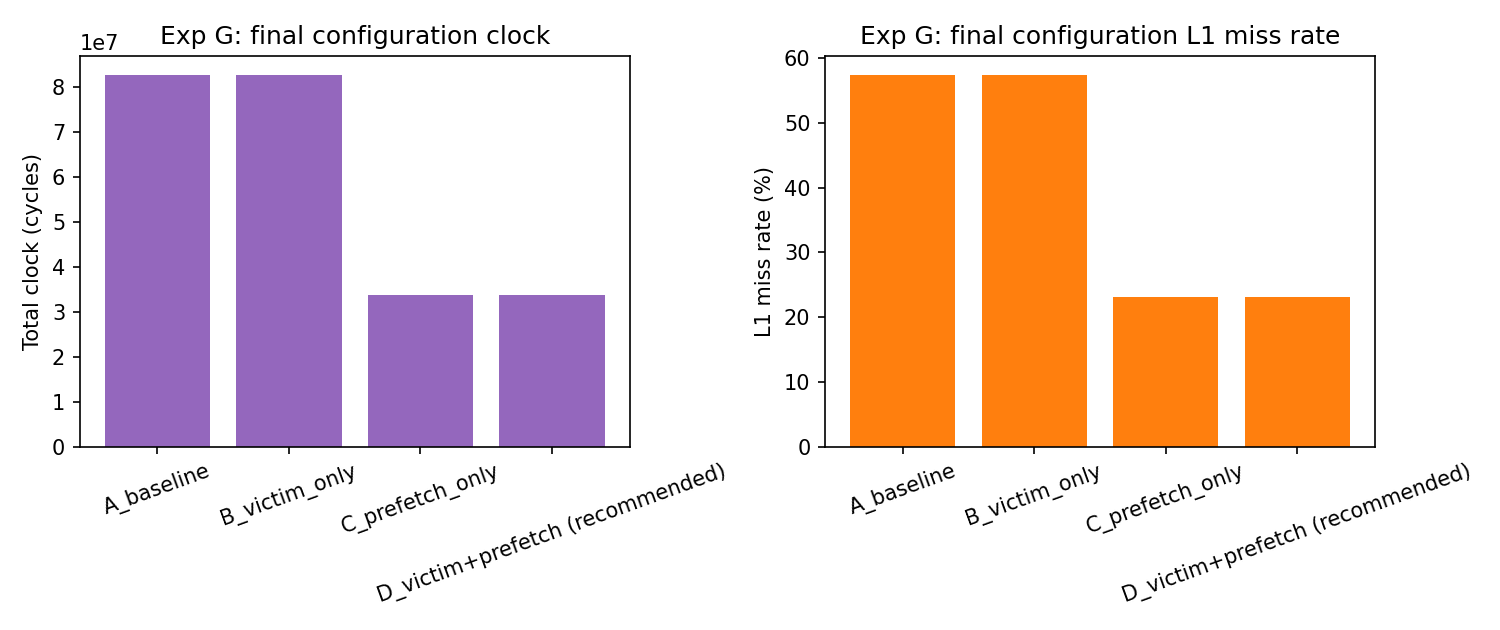
\includegraphics[width=\textwidth]{../results/plots/expG_final.png}
\caption{Final configuration comparison: execution cycles (left) and L1
miss rate (right).}
\label{fig:expG}
\end{figure}

\begin{table}[H]\centering\small
\begin{tabular}{lrrrr}\toprule
Configuration & Clock (cyc) & AMAT & L1 Miss\% & DRAM Acc. \\ \midrule
A\_baseline & 82,665,212 & 118.09 & 57.44 & 247,086 \\
B\_victim\_only & 82,658,543 & 118.08 & 57.44 & 247,086 \\
C\_prefetch\_only & 33,689,342 & 48.13 & 23.17 & 87,090 \\
D\_victim+prefetch (recommended) & 33,682,036 & 48.12 & 23.17 & 87,090 \\
\bottomrule\end{tabular}
\caption{Exp G: final configuration comparison (selected prefetcher: stream\_d16, selected victim-cache size: 64 entries).}
\label{tab:expG}\end{table}


Victim cache alone moves 82{,}665{,}212 $\to$ 82{,}658{,}543 cycles, a
0.008\% improvement, confirming Section~\ref{sec:victim}: this workload does
not offer the victim cache's target pattern at meaningful scale. Prefetch
alone moves 82{,}665{,}212 $\to$ 33{,}689{,}342 cycles, a 59.2\% reduction
and by far the dominant lever available, since Ingestion, Extraction, and
Lookup all contain enough sequential or strided structure for a well-tuned
stream prefetcher to exploit, and distance 16 sits in the zone that arrives
with time to hide the miss without meaningfully polluting. Both combined
moves 33{,}689{,}342 $\to$ 33{,}682{,}036 cycles, an additional 0.02\% on top
of prefetching alone; the victim cache's marginal contribution barely
changes once prefetching is active, for the same reason it contributed
almost nothing on its own.

\textbf{Recommendation.} Given the assignment's hardware/complexity budget,
the victim cache is not recommended for this workload: real design cost
(fully-associative tag comparators, a swap path between L1 and the victim
structure) for a measured 0.008--0.02\% return in every configuration
tested. It would be worth it only if a production version of this pipeline
were expected to hit the same-set-conflict pattern
Section~\ref{sec:victim}'s micro-benchmark isolates, for example a hash
table or index with a poor address-to-set distribution, a case this
workload as built does not trigger. A stream prefetcher at a moderate
distance (8--16) is clearly worth it: it captures most of the achievable
improvement, sits past the "too late" zone with only mild pollution cost,
and (Section~\ref{sec:pollution}) stays a strong net win even under
elevated interleave pressure. A non-blocking cache with a modest MSHR budget
(8--16) is recommended for the Result-Generation stage and any other stage
with genuine independent parallelism (Lookup's regular sub-component is a
second candidate): Section~\ref{sec:mshr} shows this captures essentially
all of the available memory-level-parallelism benefit for a workload whose
real independent-stream count is 8, with no return past that point, and
correctly no return at all for the pipeline's dependent-chain portions,
where no amount of buffering substitutes for a sequential dependency the
algorithm itself imposes.

% =====================================================================
\section{Required-Observations Checklist}
% =====================================================================

\begin{table}[H]\centering\small
\begin{tabular}{ll}\toprule
Concept & Evidence \\ \midrule
Victim Cache & \S\ref{sec:victim}, Tables~\ref{tab:expB}--\ref{tab:expB-conflict} \\
Next-Line Prefetching & \S\ref{sec:prefetch}, Table~\ref{tab:expC} (\texttt{next\_line} row) \\
Stride Prefetching & \S\ref{sec:prefetch}, Table~\ref{tab:expC} (\texttt{stride\_*} rows) \\
Stream Prefetching & \S\ref{sec:prefetch}, Table~\ref{tab:expC} (\texttt{stream\_*} rows) \\
Prefetch Distance & \S\ref{sec:distance}, Table~\ref{tab:expD}, Fig.~\ref{fig:expD} \\
Prefetch Accuracy & \S\ref{sec:prefetch}, Table~\ref{tab:expC} col.\ 3 \\
Prefetch Coverage & \S\ref{sec:prefetch}, Table~\ref{tab:expC} col.\ 4 \\
Prefetch Timeliness & \S\ref{sec:prefetch}, Table~\ref{tab:expC} col.\ 5; \texttt{stride\_d1} case \\
Prefetch Traffic & \S\ref{sec:prefetch}/\ref{sec:distance}, Table~\ref{tab:expC}/\ref{tab:expD} issued/DRAM-prefetch cols \\
Cache Pollution & \S\ref{sec:prefetch} (\texttt{stride\_d1}), \S\ref{sec:pollution} \\
Cache Thrashing & \S\ref{sec:pollution}, Table~\ref{tab:expE-baseline}; \S\ref{sec:victim} conflict micro-bench \\
Useful-Data Eviction & \S\ref{sec:distance}, \texttt{useful\_data\_evictions} in Table~\ref{tab:expD} \\
Memory-Bandwidth Pressure & \S\ref{sec:pollution} (filler traffic vs.\ agg.\ state) \\
Prefetch Interference & \S\ref{sec:pollution} (stream prefetch vs.\ agg.\ state hit rate) \\
Blocking Cache & \S\ref{sec:mshr}, MSHR\,=\,1 row of Table~\ref{tab:expF} \\
Non-Blocking Cache & \S\ref{sec:mshr}, MSHR\,$>$\,1 rows of Table~\ref{tab:expF} \\
MSHRs & \S\ref{sec:mshr} \\
Outstanding Misses & \S\ref{sec:mshr} \\
Memory-Level Parallelism & \S\ref{sec:mshr}, independent-streams curve, Fig.~\ref{fig:expF} \\
Memory-Latency Hiding & \S\ref{sec:mshr}, halving-per-MSHR-doubling result \\
\bottomrule
\end{tabular}
\caption{Where each concept required by the assignment is demonstrated with measured data.}
\end{table}

% =====================================================================
\section{Limitations}
% =====================================================================

\begin{itemize}[leftmargin=1.6em]
\item Latencies (Table~\ref{tab:sysparams}) are illustrative round numbers
for a Sapphire-Rapids-class hierarchy, not measured or vendor-published
values, which the assignment explicitly allows.
\item The blocking timing model used everywhere except Section~\ref{sec:mshr}
assumes one outstanding request at a time; absolute cycle counts there
should be read as relative comparisons under one consistent assumption, not
as absolute predicted latencies.
\item No dirty-bit/write-back state is modeled, matching the Exp-01/Exp-03
convention; a line evicted from the victim cache is simply dropped rather
than written back, assuming L2/LLC already hold a copy.
\item The 8-core / 15\,MiB-aggregate-LLC model is exercised as a
single-stream simulation against that aggregate hierarchy, per the
assignment's framing of the workload as one large-scale pipeline; true
multi-core contention for the shared LLC is out of scope here.
\item Prefetcher per-stream state is keyed on the workload generator's
logical stream tags, a simulator-level stand-in for per-PC stride tables in
real hardware, not on true instruction addresses.
\end{itemize}

% =====================================================================
\appendix
\section{Source Code}
% =====================================================================

The complete, runnable source is submitted alongside this report (four
files: \texttt{src/cache\_core.py}, \texttt{src/workload.py},
\texttt{src/mlp\_model.py}, \texttt{run\_experiments.py}). Running
\texttt{python3 run\_experiments.py} regenerates every table, CSV, JSON
file, and plot referenced above from scratch (fixed random seed, so the
numbers are exactly reproducible). All four are reproduced in full below.

\lstinputlisting[caption={\texttt{src/cache\_core.py} -- generic set-associative cache, victim cache, hierarchy simulator, and prefetcher classes}]{../src/cache_core.py}
\lstinputlisting[caption={\texttt{src/workload.py} -- the five-stage pipeline address-stream generators}]{../src/workload.py}
\lstinputlisting[caption={\texttt{src/mlp\_model.py} -- MSHR / non-blocking-cache timing model}]{../src/mlp_model.py}
\lstinputlisting[caption={\texttt{run\_experiments.py} -- experiment driver, output writers}]{../run_experiments.py}

\end{document}
